\section{Experimental Evaluation}
\label{sec:performance}

\subsection{Method and validation}

Each experimental point is the arithmetic mean of three seeds, and error bars are the sample standard deviation.  Median, extrema, coefficient of variation (CV), and per-run validation outcomes are also considered.  The measured time is end-to-end wall time around \texttt{srun}, so it includes launcher, input, initialization, solver, output, and finalization.  Open MPI 4.1.6 and \texttt{-O3} are visible in the logs; CPU and GPU model identifiers are not.

Every current CSV row has positive finite timing and a matching solution file.  Reconstructed routes visit every customer exactly once and satisfy capacity.  Seven multi-rank outputs have a feasible printed route whose recomputed cost differs from the printed scalar best cost; their timings are retained, but their costs are excluded.  MPI RSS values are also excluded because \texttt{/usr/bin/time} observed the \texttt{srun} launcher rather than remote ranks.

\subsection{Strong scaling}

The strong experiment fixes $n=32{,}000$, $K=32$, the total population at $m=16$, and the work at 100 epochs; stagnation is disabled.  OpenMP measurements use one MPI rank and up to 32 threads, while the distributed measurement uses four ranks with 32 threads per rank.  We define $p=\text{ranks}\times\text{threads}$, $S_p=T_1/T_p$, and $E_p=S_p/p$.

\begin{figure*}[t]
\centering
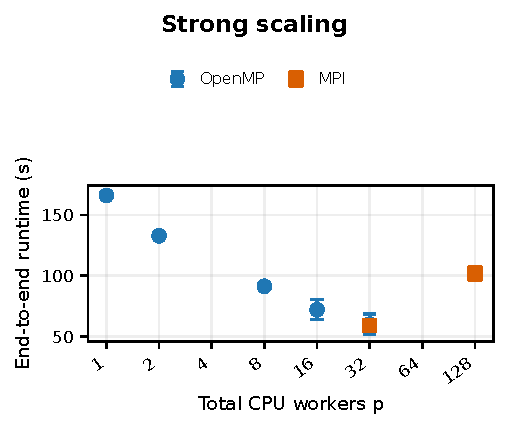
\includegraphics[width=0.32\textwidth]{figures/scaling/strong_scaling_runtime.pdf}\hfill
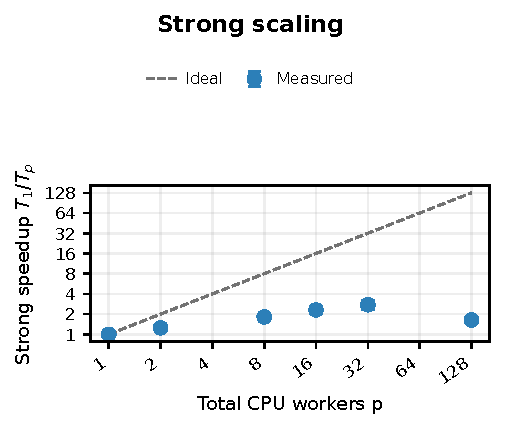
\includegraphics[width=0.32\textwidth]{figures/scaling/strong_scaling_speedup.pdf}\hfill
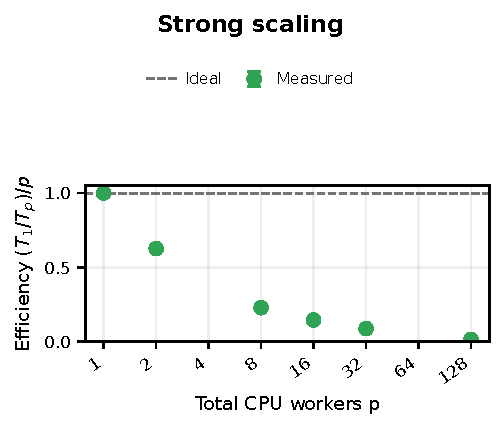
\includegraphics[width=0.32\textwidth]{figures/scaling/strong_scaling_efficiency.pdf}
\caption{Strong-scaling runtime, speedup, and efficiency as three distinct plots. Points show means of three runs; runtime bars are sample SD and ratio bars use first-order SD propagation. The combined curves use OpenMP within one node and the four-rank MPI result at 128 workers.}
\label{fig:strong-current}
\end{figure*}

Mean OpenMP runtime falls from $165.98\pm2.11$~s at one thread to $60.09\pm8.39$~s at 32 threads.  The corresponding speedup is only $2.76$ and efficiency is $8.63\%$; variability also grows to a CV of $13.96\%$.  The fixed population explains an important part of this behavior: the ant-construction loop exposes only 16 independent ants per epoch, so at 32 threads at least half of the workers cannot receive an ant-construction task.  Additional threads can still accelerate dense evaporation and other parallel loops, but they do not increase concurrency in the principal coarse-grained phase.  End-to-end initialization, phase barriers, atomic deposits, and dense-matrix traffic further bound the attainable speedup.  The measurements therefore show insufficient task granularity for this strong-scaling configuration, while profiling would be needed to quantify the contribution of each remaining phase.

The independent 32-worker MPI baseline is $59.00\pm3.77$~s, compatible in scale with the OpenMP 32-thread measurement.  Four ranks require $101.60\pm5.60$~s.  Relative to the 32-worker MPI point this is a speedup of $0.58$ and an efficiency of $14.5\%$ after normalizing by the fourfold resource increase.  Relative to the one-thread combined baseline, the 128-worker point has speedup $1.63$ and efficiency $1.28\%$.  Here the 16 ants are divided among four ranks, leaving only four local ants for 32 OpenMP threads on each rank during construction.  At the same time, every rank stores and evaporates its dense pheromone replica and participates in collective coordination.  The added resources thus increase replicated and coordination work without adding ant work, which accounts for the direction of the observed slowdown; a phase profile would still be required to apportion its magnitude.

\subsection{Weak scaling}

The weak campaign fixes $n=8{,}000$ and 100 epochs while maintaining 32 ants per total CPU worker.  OpenMP covers 1--32 workers on one rank; MPI extends the curve to 64 and 128 workers with 32 threads per rank.  The population therefore grows from 32 to 4096 and the workload-per-worker relation is constant.  I report $E^{weak}_p=T_1/T_p$ and use the OpenMP point at 32 workers in the combined curve.  The independent one-rank MPI measurement at the same point is retained as a consistency check.

\begin{figure*}[t]
\centering
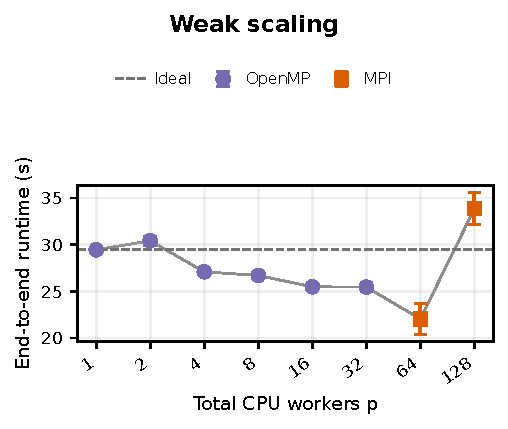
\includegraphics[width=0.48\textwidth]{figures/scaling/weak_scaling_runtime.pdf}\hfill
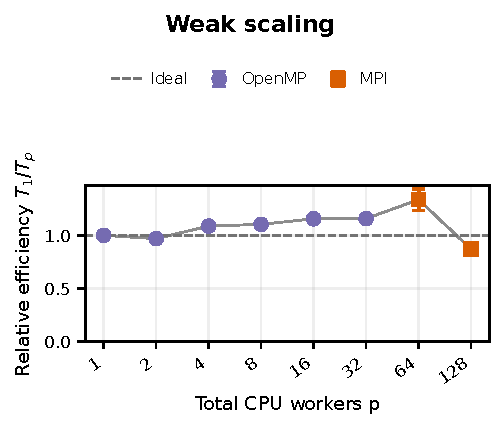
\includegraphics[width=0.48\textwidth]{figures/scaling/weak_scaling_efficiency.pdf}
\caption{Weak-scaling runtime and efficiency as distinct plots. OpenMP supplies 1--32 workers and MPI supplies 64--128. Points are three-run means with sample-SD bars; efficiency is $T_1/T_p$.}
\label{fig:weak-current}
\end{figure*}

Runtime is $29.46\pm0.10$~s at one worker, remains between $25.47$ and $30.43$~s through 32 OpenMP workers, falls to $22.05\pm1.65$~s at 64, and rises to $33.87\pm1.70$~s at 128.  Weak efficiency is $1.16$ at 32, $1.34$ at 64, and $0.87$ at 128.  The 32-worker MPI control is $25.42\pm0.65$~s versus $25.47\pm0.44$~s for OpenMP, supporting continuity at the backend transition.  Unlike strong scaling, this campaign supplies 32 ants per worker, so the coarse-grained loop remains populated as resources grow.  This directly explains why weak efficiency is much better than strong efficiency.  Ratios above one are consistent with amortization of fixed phase costs, but cache, scheduling, and hardware effects cannot be separated without profiling.

\subsection{Sequential and CUDA size sweep}

The size sweep covers sequential runs through $n=32{,}000$ and CUDA through $n=64{,}000$.  It is not a like-for-like speedup experiment: CUDA uses $m=256$, while the sequential population varies from 32 to 4, and both stop on stagnation or at 300 solver seconds.  Sequential runs hit the time limit from $n=2{,}000$ onward; CUDA hits it at $n=64{,}000$.  External times can exceed 300~s because initialization and finalization are outside the solver timer.

\begin{figure}[H]
\centering
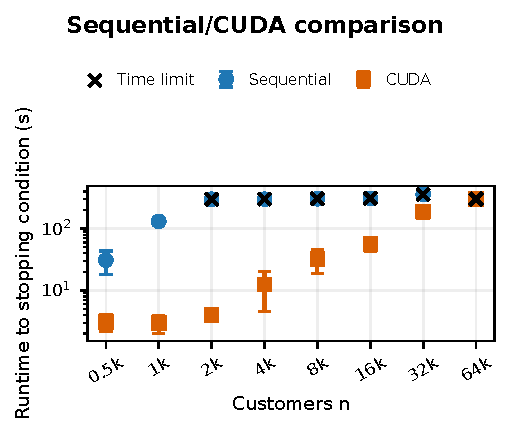
\includegraphics[width=\columnwidth]{figures/comparison/backend_runtime.pdf}
\caption{Runtime in the descriptive size sweep. Points are three-run means with sample-SD bars; crosses mark time-limited groups.}
\label{fig:backend-current}
\end{figure}

\begin{figure}[H]
\centering
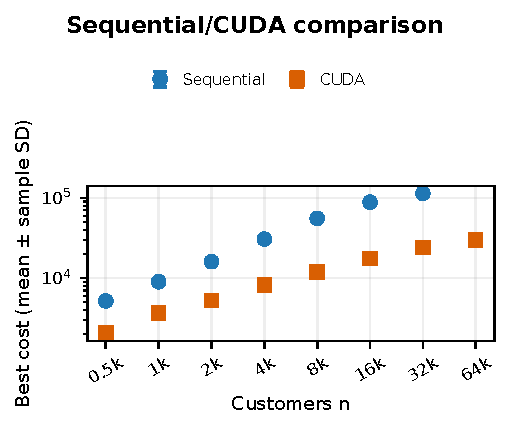
\includegraphics[width=\columnwidth]{figures/comparison/backend_cost.pdf}
\caption{Cost in the descriptive size sweep. Points are three-run means with sample-SD bars. Different populations and stopping epochs preclude interpreting the comparison as a backend speedup.}
\label{fig:backend-cost}
\end{figure}

CUDA reaches $n=64{,}000$ within the available outputs, while the dense sequential backend reaches $n=32{,}000$ with about 26.7~GiB RSS.  Runtime variability is substantial for several stagnation-terminated CUDA points (CV $62.9\%$ at $n=4{,}000$ and $41.8\%$ at $n=8{,}000$), so a single best run would be misleading.  Although CUDA reports lower runtime and cost on all shared sizes, the unequal search effort means that these observations cannot establish an implementation speedup or equal-budget quality advantage.

\section{Conclusions}

The reliable current evidence supports three limited conclusions.  First, OpenMP reduces the 100-epoch runtime on the $n=32{,}000$ instance, but a population of only 16 ants leaves the 32-thread configuration underutilized and limits speedup to $2.76\times$.  Second, splitting the same fixed population over four MPI ranks increases replicated and collective work while leaving only four ants per rank, producing a multi-node slowdown.  In contrast, the weak campaign keeps enough independent ants per worker and preserves $87\%$ efficiency at 128.  Third, the CUDA representation handles the largest available instance, but the present size sweep is not controlled well enough for a cross-backend speedup claim.

These results characterize the submitted configuration rather than a general limit of OpenMP or MPI.  Its strong-scaling resource count grows beyond the available ant-level parallelism, whereas the weak campaign grows useful work with the worker count.  Hardware identifiers, rank-level memory measurements, and phase profiling would be necessary for a more detailed attribution.  The inconsistent transfer of the globally best MPI route also remains a correctness limitation for quality comparisons, although its fixed-work timings are retained.

\vspace{-0.75\baselineskip}
{\small
\begin{thebibliography}{9}
\bibitem{wiki-vrp} Wikipedia, \emph{Vehicle routing problem}: \url{https://en.wikipedia.org/wiki/Vehicle_routing_problem}
\bibitem{wiki-aco} Wikipedia, \emph{Ant colony optimization algorithms}: \url{https://en.wikipedia.org/wiki/Ant_colony_optimization_algorithms}
\end{thebibliography}
}
